\documentclass[11pt,a4paper]{article}
\usepackage[a4paper,margin=2.0cm]{geometry}
\usepackage[T1]{fontenc}\usepackage[utf8]{inputenc}\usepackage{lmodern}
\usepackage{amsmath,amssymb}
\usepackage{booktabs,array,multirow,longtable}
\usepackage{enumitem}
\usepackage{xcolor}
\usepackage{graphicx}
\usepackage{caption}
\captionsetup{font=small,labelfont=bf}
\usepackage{tcolorbox}
\usepackage{needspace}
\usepackage[hidelinks]{hyperref}
\newcommand{\un}[1]{\,\mathrm{#1}}
\newtcolorbox{warn}{colback=red!4,colframe=red!60!black,boxrule=0.6pt,arc=2pt,left=4pt,right=4pt,top=3pt,bottom=3pt,fontupper=\small}
\newtcolorbox{tip}{colback=green!4,colframe=green!45!black,boxrule=0.6pt,arc=2pt,left=4pt,right=4pt,top=3pt,bottom=3pt,fontupper=\small}
\newtcolorbox{why}{colback=blue!4,colframe=blue!50!black,boxrule=0.6pt,arc=2pt,left=4pt,right=4pt,top=3pt,bottom=3pt,fontupper=\small}

\title{\vspace{-1.5cm}Experimental plan for the redo\\[2pt]\large Coupled magnetic--mechanical oscillator: one run of $8$ separations $\times$ $5$ trials}
\author{}
\date{Planning document, version 3 --- numbers are \emph{predictions} from the first data set after the time-base correction of \S0 ($f_1=6.49\un{Hz}$, $C=1.33\times10^{-7}\un{m^5\,s^{-2}}$, $\tau\approx21\un{s}$); they will be replaced by the measured values}

\begin{document}
\maketitle
\vspace{-1.2cm}

\section*{0. First: the time base --- everything in run 1 was 8 times too slow}

Your new FFT (clip set to $240\un{s^{-1}}$ in Clip Settings) puts the main peak at $6.51\un{Hz}$, with the second one at $\approx8.3\un{Hz}$; run 1 gave $0.811\un{Hz}$ for the same spring. $6.51/0.811=8.03$. The explanation is not physics: a 240 fps slow-motion file is \emph{stored} for playback at 30 fps, and Tracker reads that playback rate unless the frame rate is typed into Clip Settings. Run 1 was analysed with the file's 30 fps, so every time was stretched by $240/30=8$ and every frequency divided by 8. The springs really oscillate at $\approx6.5\un{Hz}$ (6 s of your record contain about 40 swings --- count them), and the pair beats about once per second at this $d$, which is what you saw: many beats in 6 s.

What this changes and what it does not:
\begin{itemize}[leftmargin=1.6em,itemsep=1pt]
\item \textbf{Unchanged}: every ratio. $f_2/f_1$, $2\gamma/k$, the exponent of the $\ln$--$\ln$ graph ($-3.75$ in run 1), the static bend $\delta$, $x_{20}$, the non-linear shifts in \%, the equal-amplitude prediction, all Tracker advice. The run-1 data stay valid --- multiply all their frequencies by 8.
\item \textbf{Rescaled}: $f_1=0.811\to6.49\un{Hz}$; $C=(f_2^2-f_1^2)d^5$ becomes $64\times$ larger, $1.33\times10^{-7}\un{m^5\,s^{-2}}$; $k/m=\omega_1^2$ becomes $64\times$ larger ($1660\un{s^{-2}}$); the decay time $\tau\approx170\un{s}$ becomes $\approx21\un{s}$; every beat period is 8 times shorter. So the records of the previous version of this plan (60--400 s) were 8 times too long, and the ``soft spring'' and gravity discussion shrinks to a few-per-cent side issue (\S2).
\item \textbf{Check it once more} before the redo: in Clip Settings the frame rate must read $240$ and the frame dt $4.17\times10^{-3}\un{s}$ for every clip (import the first clip's \texttt{.trk} into the others, \S3). Say so explicitly in the essay's method --- it is exactly the kind of systematic check examiners reward.
\end{itemize}

\section{What is measured and why}

\begin{center}\small
\begin{tabular}{@{}p{3.5cm}p{4.9cm}p{7.2cm}@{}}
\toprule
quantity & how & used for\\
\midrule
$f_1,\ f_2$ at each $d$ & FFT of $x_1(t)$ and $x_2(t)$ from Tracker; also FFT of $x_1\!+\!x_2$ and $x_1\!-\!x_2$ & main graph $\ln(f_2^2-f_1^2)$ vs $\ln d$ (gradient $-5$); $f_{\rm avg}$, $f_{\rm beat}$\\
$d$ (centre to centre) & $d=g+t$: gap $g$ between magnet faces (digital calliper / photo with scale) $+$ magnet thickness $t$ & independent variable\\
$f_a,\ f_b$ & each spring plucked alone (other magnet removed) & identical-spring check, detuned model, gives $k/m$\\
$k$ & static load--deflection graph (\S6) & absolute test of $C$; non-linear model\\
$M,\ \mu L$ & balance & effective mass $m=M+\tfrac{33}{140}\mu L$, cross-check of $m=k/\omega_1^2$\\
$L,\ b,\ h$ & ruler / calliper / micrometer & $k=Ebh^3/4L^3$ cross-check (with the small gravity term of \S2); Rayleigh factor\\
magnet $D,\ t,\ B_{\rm r}$ or $\mu_{\rm m}$ & calliper; data sheet or pull-force / Hall probe & $\mu_{\rm m}\approx B_{\rm r}V/\mu_0$, finite-size correction\\
\bottomrule
\end{tabular}
\end{center}

\begin{why}
\textbf{Why $f_2^2-f_1^2$.} Subtracting the two mode results $\omega_1^2=k/m$, $\omega_2^2=(k+2\gamma)/m$ removes $k$: $f_2^2-f_1^2=\gamma/2\pi^2m=Cd^{-5}$. The \emph{exponent} therefore needs only frequencies and $d$; $k$, $m$ and $\mu_{\rm m}$ are needed only for the absolute value of $C$. Angular frequencies are not required anywhere ($\omega=2\pi f$ cancels in every ratio), so the FFT frequencies can be used directly; convert to $\omega$ only if you want to quote $k/m=\omega_1^2$.
\end{why}

\section{Apparatus and set-up}

\begin{enumerate}[leftmargin=1.6em,itemsep=2pt]
\item \textbf{Base and clamps.} Non-magnetic base (wood/aluminium), two clamps. Mark the base with a mm scale or fix a steel rule \emph{behind the plane of the magnets} (out of the plane, so it does not attract them).
\item \textbf{Springs.} Two strips from the same stock (same $b$ and $h$ --- check $h$ with a micrometer, $k\propto h^3$), same free length $L$ above the clamp jaws. Which of your lengths to use is decided by the \emph{single-spring frequency} $f_a$, not by $L$ itself --- see ``Which spring length'' below; the strip you have been using ($f_a\approx6.5\un{Hz}$) is fine. Measure $L$ from the top of the jaw to the \emph{centre of the magnet}; write down $L$ before every session because re-clamping changes it.
\item \textbf{Magnets.} Glue (or double-sided tape) each magnet flat on the \emph{inner face} of the strip with its centre a few mm below the tip, like poles facing. It does \emph{not} have to be exactly at the very tip --- what matters is that (i) both are at the same height, (ii) the strip length is quoted to the magnet centre, (iii) the position never changes between runs. Put a small high-contrast dot (white marker / sticker) on the visible side of each magnet: this is what Tracker follows.
\item \textbf{Alignment.} Magnets coaxial: same height ($\pm1\un{mm}$), same depth from the camera, faces parallel. Check by eye from above and from the front.
\item \textbf{Camera.} Phone on a tripod, lens at the height of the magnets, $\ge0.8\un{m}$ away and \emph{square} to the plane of motion (parallax otherwise turns a straight motion into a curved one). Zoom until the two magnets plus $\approx30\un{mm}$ on either side fill the frame width. Fix focus and exposure (tap and hold). Bright, even light; no flicker (LED/daylight, avoid old fluorescent tubes at 240 fps).
\item \textbf{Scale.} A ruler in the plane of the magnets, visible in every video (calibration stick in Tracker). Since $d$ is measured with a calliper this scale only sets the mm/pixel factor for amplitudes.
\end{enumerate}

\begin{warn}
\textbf{Things that silently ruin a run:} magnets glued at different heights (they stop being coaxial and $F$ is no longer along $x$); a steel rule, steel clamp screw or the phone's own magnet within a few cm of the magnets; the clamps loosening between trials ($f_1$ drifts --- re-measure the ``Infinity'' frequency at the end of the session); camera not square to the motion.
\end{warn}

\subsection*{Which spring length?}\label{box:length}
The magnets do not care about $L$; they care about how stiff each strip is compared with the magnetic stiffness, i.e.\ about the \emph{frequency of one spring alone with its magnet}, $f_a$. Every prediction in this plan depends on $f_a$ only, so compare your strips by $f_a$, not by length: attach one magnet (or Blu-Tack of the same mass), clamp the strip, film 10 s, FFT in Tracker. Only the \emph{free} length above the jaws counts, so a long strip can always be clamped shorter; what you cannot fix afterwards is a thickness difference, so both strips must come from the same stock. With the magnets of run~1 and the ladder of \S3 (records of 45 s), this is what each $f_a$ gives:
\begin{center}\footnotesize
\setlength{\tabcolsep}{4pt}
\begin{tabular}{@{}lccccccc@{}}
\toprule
$f_a$ / Hz & $L/L_{\rm run\,1}$ & \begin{tabular}[c]{@{}c@{}}$f_2-f_1$\\ at 24.5 mm\end{tabular} & \begin{tabular}[c]{@{}c@{}}$f_2-f_1$\\ at 42 mm\end{tabular} & \begin{tabular}[c]{@{}c@{}}$T_{\rm beat}$\\ at 42 mm\end{tabular} & \begin{tabular}[c]{@{}c@{}}largest\\ usable $d$\end{tabular} & \begin{tabular}[c]{@{}c@{}}$2\gamma/k$\\ at 24.5 mm\end{tabular} & \begin{tabular}[c]{@{}c@{}}$\delta$\\ at 24.5 mm\end{tabular}\\
\midrule
4.5 & 1.28 & 1.44 Hz & 112 mHz & 9.0 s & 46 mm & 0.74 & 2.3 mm\\
5.0 & 1.19 & 1.33 Hz & 101 mHz & 9.9 s & 45 mm & 0.60 & 1.8 mm\\
\textbf{5.5} & \textbf{1.12} & 1.23 Hz & 92 mHz & 10.9 s & 44 mm & 0.50 & 1.5 mm\\
\textbf{6.5 (run 1)} & \textbf{1.00} & 1.07 Hz & 78 mHz & 12.9 s & 42 mm & 0.36 & 1.1 mm\\
8.0 & 0.87 & 0.89 Hz & 63 mHz & 15.8 s & 41 mm & 0.24 & 0.7 mm\\
10.0 & 0.75 & 0.73 Hz & 51 mHz & 19.7 s & 39 mm & 0.15 & 0.5 mm\\
\bottomrule
\end{tabular}
\end{center}
(``largest usable $d$'': where $3T_{\rm beat}$ reaches the 45 s record; $L/L_{\rm run\,1}$ from $f\propto L^{-3/2}$, approximate because the strip's own mass also changes with $L$.)

\textbf{Recommendation: keep the strip you have ($f_a\approx6.5\un{Hz}$), or go at most one step softer ($f_a\approx5$--$5.5\un{Hz}$, $\approx10$--$15\,\%$ longer).} Softer strips give a larger splitting at every $d$ (the magnetic stiffness is a larger fraction of $k$) and so a slightly wider usable range, but the gain from 6.5 to 5.5 Hz is only $15\,\%$, while $\delta$ and $x_{20}$ grow and the strip is easier to disturb. Below $f_a\approx4.5\un{Hz}$ the closest point is no longer weakly coupled ($2\gamma/k\to1$, $\delta>2\un{mm}$). Stiffer strips ($f_a\ge8\un{Hz}$) shrink the effect everywhere and lose the last ladder points. The strongest argument for keeping the present strip is continuity: run 1 (frequencies $\times8$) then becomes a genuine pilot study in the essay, directly comparable with the redo.

\begin{why}
\textbf{Gravity, for completeness.} A vertical strip with a tip magnet is an inverted pendulum: gravity reduces the stiffness, $k_{\rm eff}=k-(1.2M+0.375\,\mu L)\,g/L$ (tip-load shape; setting $k_{\rm eff}=0$ gives the Euler buckling load to $1\,\%$). At $f_a=6.5\un{Hz}$ the correction is $(1.2$--$1.6)\,g/(L\omega_a^2)\approx3$--$6\,\%$ of $k$ for $L=0.15$--$0.25\un{m}$ --- worth one sentence when $k=Ebh^3/4L^3$ is compared with the measured $k$, and the reason for measuring $k$ with the strip vertical and the magnet on (\S6), but nothing to design around. (In the previous version of this plan, with the 8-times-too-low frequencies, the same formula made gravity cancel two thirds of $k$; that was an artefact of the time base.) Since $f_a\propto L^{-3/2}$, a $1\,\%$ difference in $L$ or $0.3\,\%$ in $h$ detunes the pair by $1.5\,\%$ or $1\,\%$: tune the pair by sliding one strip in its clamp (\S4).
\end{why}

\section{Separations, amplitude and record length}

\subsection*{Which separations}
Choose them roughly \emph{evenly spaced in $\ln d$} (equal steps on the log--log graph), from the closest the clamps allow (you measured $24.5\un{mm}$) to the largest $d$ at which the two peaks are still separated in a record of practical length. Eight values ($\approx8\,\%$ steps), predictions for $f_1=6.49\un{Hz}$:
\begin{center}\small
\begin{tabular}{@{}lcccccccc@{}}
\toprule
$d$ / mm (target) & 24.5 & 26.5 & 28.5 & 31 & 33.5 & 36 & 39 & 42\\
predicted $f_2$ / Hz & 7.56 & 7.23 & 7.01 & 6.84 & 6.73 & 6.66 & 6.60 & 6.57\\
predicted $f_2-f_1$ / Hz & 1.07 & 0.74 & 0.52 & 0.35 & 0.24 & 0.17 & 0.11 & 0.078\\
predicted $T_{\rm beat}$ / s & 0.93 & 1.35 & 1.9 & 2.9 & 4.2 & 6.0 & 8.9 & 12.8\\
minimum ($3T_{\rm beat}$) / s & 2.8 & 4.0 & 5.7 & 8.6 & 12.6 & 18 & 27 & 39\\
\textbf{record length} / s & \textbf{45} & \textbf{45} & \textbf{45} & \textbf{45} & \textbf{45} & \textbf{45} & \textbf{45} & \textbf{45}\\
beats in the record & 48 & 33 & 24 & 16 & 11 & 7.5 & 5 & 3.5\\
$\pm\frac12$-bin error on $f_2^2-f_1^2$ (naive FFT) & 1.5\,\% & 2.1\,\% & 3.0\,\% & 4.5\,\% & 6.6\,\% & 9\,\% & 14\,\% & 20\,\%\\
static outward bend $\delta$ / mm & 1.1 & 0.8 & 0.6 & 0.43 & 0.31 & 0.23 & 0.17 & 0.13\\
\bottomrule
\end{tabular}
\end{center}
With the real time base one record length serves all points: $45\un{s}$ ($10\,800$ frames at 240 fps) is $\ge3T_{\rm beat}$ everywhere, and longer is pointless because the amplitude has decayed to $\approx10\,\%$ by then ($\tau\approx21\un{s}$; the FFT peak width is then set by the damping, $\sqrt3/\pi\tau\approx0.026\un{Hz}$, not by $1/T$). A constant $T$ is convenient (the same bin width, $1/T=0.022\un{Hz}$, for all $d$, so one uncertainty column) but \emph{not} required: the rule is $T\ge3T_{\rm beat}$ at each point, and the uncertainty is computed from the $T$ actually analysed. A 35 s record at 24.5 mm (37 beats, 0.029 Hz bins) is more than enough and does not need repeating; only the 39 and 42 mm points genuinely need $\ge30$--$40$ s. Do not extend the ladder beyond $\approx44\un{mm}$: from $45\un{mm}$ on even a Hann-windowed 45 s record no longer separates the peaks (the single-peak points of run 1 at $45$--$60\un{mm}$ were this limit, not a discovery).

The exact values do not matter (you cannot set $d$ precisely anyway because the springs bend outwards by $\delta$ when the second magnet is mounted): set the clamps, \emph{then measure $d$ as it is}. Do not go below $d\approx2D$ ($D$ = magnet diameter; dipole approximation) or below $g\approx8\un{mm}$.

\begin{tip}
\textbf{One trick to reach smaller $d$ if you want it.} The clamps limit the \emph{clamp} spacing $d_0$, not $d$. Mount the magnets on the \emph{inner} faces (already planned) and, if the clamp jaws are wide, offset each strip towards the inner edge of its jaw. Alternatively clamp the two strips in one wide clamp with a spacer block between them: $d_0=$ spacer $+\,h$.
\end{tip}

\begin{tip}
\textbf{Ladder order.} Do the eight separations in \emph{random} order, not from small to large, and mark the clamp positions on the base so that a spoiled point can be repeated. Move only clamp~2 to change $d$; clamp~1, the camera and the amplitude stop then stay where they are. One trial of each $d$ first, then the remaining four --- if something is wrong you find out after 8 videos, not 40.
\end{tip}

\subsection*{Release amplitude}
Pull spring 1 \emph{outwards} (away from spring 2) by $A=5\un{mm}$ at the magnet, against a stop or a mark (below), hold still for $\approx2\un{s}$ (spring~2 settles), release. Same $A$ in every trial: $A$ is a controlled variable because the non-linear force shifts $f_2$ by an amount that depends on the amplitude:
\begin{center}\small
\begin{tabular}{@{}lcccccccc@{}}
\toprule
$d$ / mm & 24.5 & 26.5 & 28.5 & 31 & 33.5 & 36 & 39 & 42\\
$f_2$ shift, $A=5\un{mm}$ & $+1.2\,\%$ & $+0.9\,\%$ & $+0.7\,\%$ & $+0.4\,\%$ & $+0.3\,\%$ & $+0.2\,\%$ & $+0.1\,\%$ & $+0.06\,\%$\\
$f_2$ shift, $A=10\un{mm}$ & $+4.6\,\%$ & $+3.7\,\%$ & $+2.8\,\%$ & $+1.8\,\%$ & $+1.2\,\%$ & $+0.8\,\%$ & $+0.5\,\%$ & $+0.3\,\%$\\
\bottomrule
\end{tabular}
\end{center}
(anti-phase mode with separation swing $\pm A$; simulated with the full $r^{-4}$ force; percentages independent of the time base). $A=5\un{mm}$ keeps this at or below the FFT uncertainty except at the two closest points, while still giving $\approx100$ pixels of motion if the frame width is $\approx120\un{mm}$; the residual shift is exactly what the non-linear model in the evaluation predicts, so it becomes a test rather than an error. Why outwards: pulling apart lowers the repulsion during the hold, so spring~2 is not pushed off-axis and the magnets can never touch.

\paragraph{How to pull by 5 mm without Tracker.} Tracker is never needed \emph{during} the session: it is run once, afterwards, on the 40 clips, and if the tripod is not moved a single calibration stick and set of axes serve all clips (analyse the first clip, save the \texttt{.trk}, then \textsf{File $\triangleright$ Import $\triangleright$ Tracker file} to bring the calibration and axes into each new clip). Nor should you measure the gap between the two tips while pulling --- spring~2 follows spring~1 by $x_{20}=A\gamma/(k+\gamma)$ ($\approx0.8\un{mm}$ at $24.5\un{mm}$, $\approx0.06\un{mm}$ at $42\un{mm}$), so the tip-to-tip distance grows by more than $A$ and by a different amount at each $d$. Reference spring~1 to the base instead:
\begin{itemize}[leftmargin=1.6em,itemsep=1pt]
\item \textbf{Recommended: a stop set once per separation with a 5 mm gauge.} Fix a small post on the base outside spring 1, at magnet height (a bolt in a slotted bracket, a block on Blu-Tack, or a wooden dowel in a clip --- anything non-magnetic that you can slide and fix). After the clamps are set and both springs are at rest, lock a calliper at $5.00\un{mm}$ and use its inside jaws (or a $5\un{mm}$ drill shank / stack of card measured with the calliper) as a gauge: hold it against the outer face of strip 1, push the post up to the gauge, fix the post, remove the gauge. Time: 20 s, once per $d$ (the rest position of strip 1 shifts by up to $1\un{mm}$ between separations because $\delta$ changes, so the post must be re-set each time $d$ changes, but not between trials). Every trial is then: pull strip 1 against the post with two fingertips, hold 2 s, open the fingers. $A$ is identical for the five trials to $\pm0.1\un{mm}$ with nothing to read or aim at. After release the strip can never reach the post again: its outward excursion is bounded by $A$ (energy argument --- the initial state is the one with all the energy in the springs) and damping plus the imperfect re-alignment of the two modes keep the closest return a few tenths of a millimetre short, arriving at zero velocity. Check the first clip at $24.5\un{mm}$ anyway (closest return, at the first beat maximum) and glue a scrap of felt on the post face if you ever see a tap.
\item \textbf{Alternative: two pencil marks.} A card fixed behind magnet~1 (in the plane of the tracked dot) with a mm scale or two marks 5 mm apart; note the rest reading once per $d$, pull until the dot is at rest $-5$. Sighting error $\approx0.5\un{mm}$ ($10\,\%$ of $A$) is harmless: $A$ affects only the peak heights and the small non-linear shift ($\propto A^2$: $\pm10\,\%$ in $A$ moves $f_2$ at $24.5\un{mm}$ by $\pm0.25\,\%$, less elsewhere), never $f_1$.
\item Pull \emph{at the magnet height}, not half-way down the strip (so the strip shape is the static tip-load curve assumed by the theory), and pull with fingertips on the outer face so that the release is an opening of the fingers, never a push.
\item The actual $A$ of every trial comes free with the analysis --- it is the first maximum of $x_1(t)$ after release --- and is what you report in the data table; the stop or the marks only guide your hand.
\end{itemize}

\subsection*{Frame rate and record length}
\begin{itemize}[leftmargin=1.6em,itemsep=1pt]
\item \textbf{240 fps is right and now clearly needed}: at $6.5$--$7.6\un{Hz}$ it gives 32--37 frames per oscillation; 30 fps would give only 4--5. In Tracker use \textbf{step size 2} (120 fps, 16--18 points per swing; the dot moves $\le2\un{mm}$ between analysed frames, so the autotracker never loses it); step size 4 (8--9 points per swing) is still enough for the frequencies but marginal for the tracker at $A=5\un{mm}$. Type $240$ into Clip Settings for every clip (\S0).
\item \textbf{Record length: 45 s for every $d$}: camera on, 3 s rest, pull, hold 2 s, release, then $\approx45\un{s}$; stop at about one minute of video. The requirement is $T\ge3T_{\rm beat}$ (three swellings) \emph{and} a resolution good enough for the smallest splitting: with $T=45\un{s}$ the bin width is $0.022\un{Hz}$, versus $f_2-f_1=0.078\un{Hz}$ at $42\un{mm}$ (3.5 bins). Your 6 s record is \emph{not} short because of the beats --- it contains six of them --- it is short because a 6 s record has $0.17\un{Hz}$ bins: even at $24.5\un{mm}$ the naive peak position is uncertain by $\pm0.08\un{Hz}$, i.e.\ $\pm11\,\%$ on $f_2^2-f_1^2$, and at $42\un{mm}$ the two peaks are one blob (Fig.~2). Beyond $\approx50\un{s}$ nothing is gained: the amplitude is down to $10\,\%$ and the peak width is set by the damping.
\item Quote $T$ (the analysed window, starting $\approx1\un{s}$ after release) per point in the data table; it need not be the same for all points, but every point must satisfy $T\ge3T_{\rm beat}$.
\end{itemize}

\begin{figure}[!tb]\centering
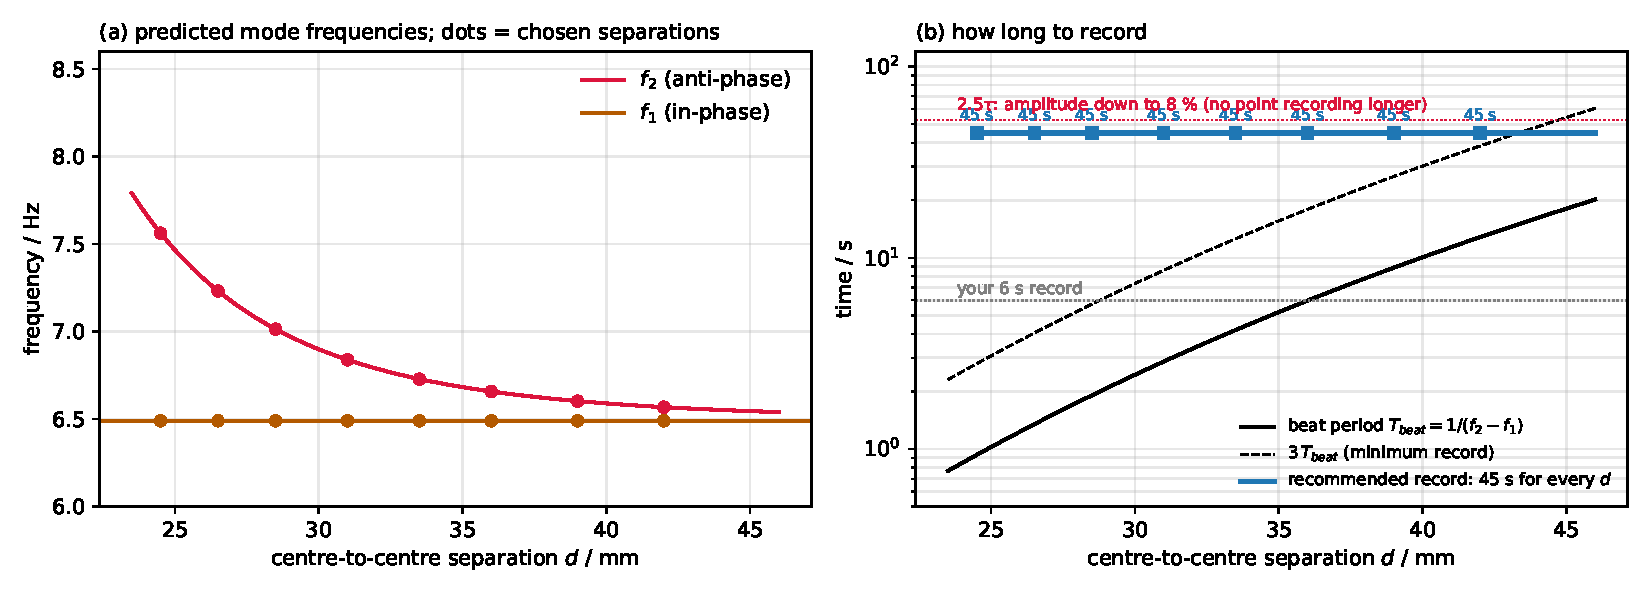
\includegraphics[width=0.86\textwidth]{design_plot.pdf}
\caption{(a) Predicted mode frequencies at the chosen separations (real time base). (b) Beat period, the ``three beats'' minimum, the 45 s record, and the decay limit $2.5\tau$.}
\end{figure}

\begin{figure}[!tb]\centering
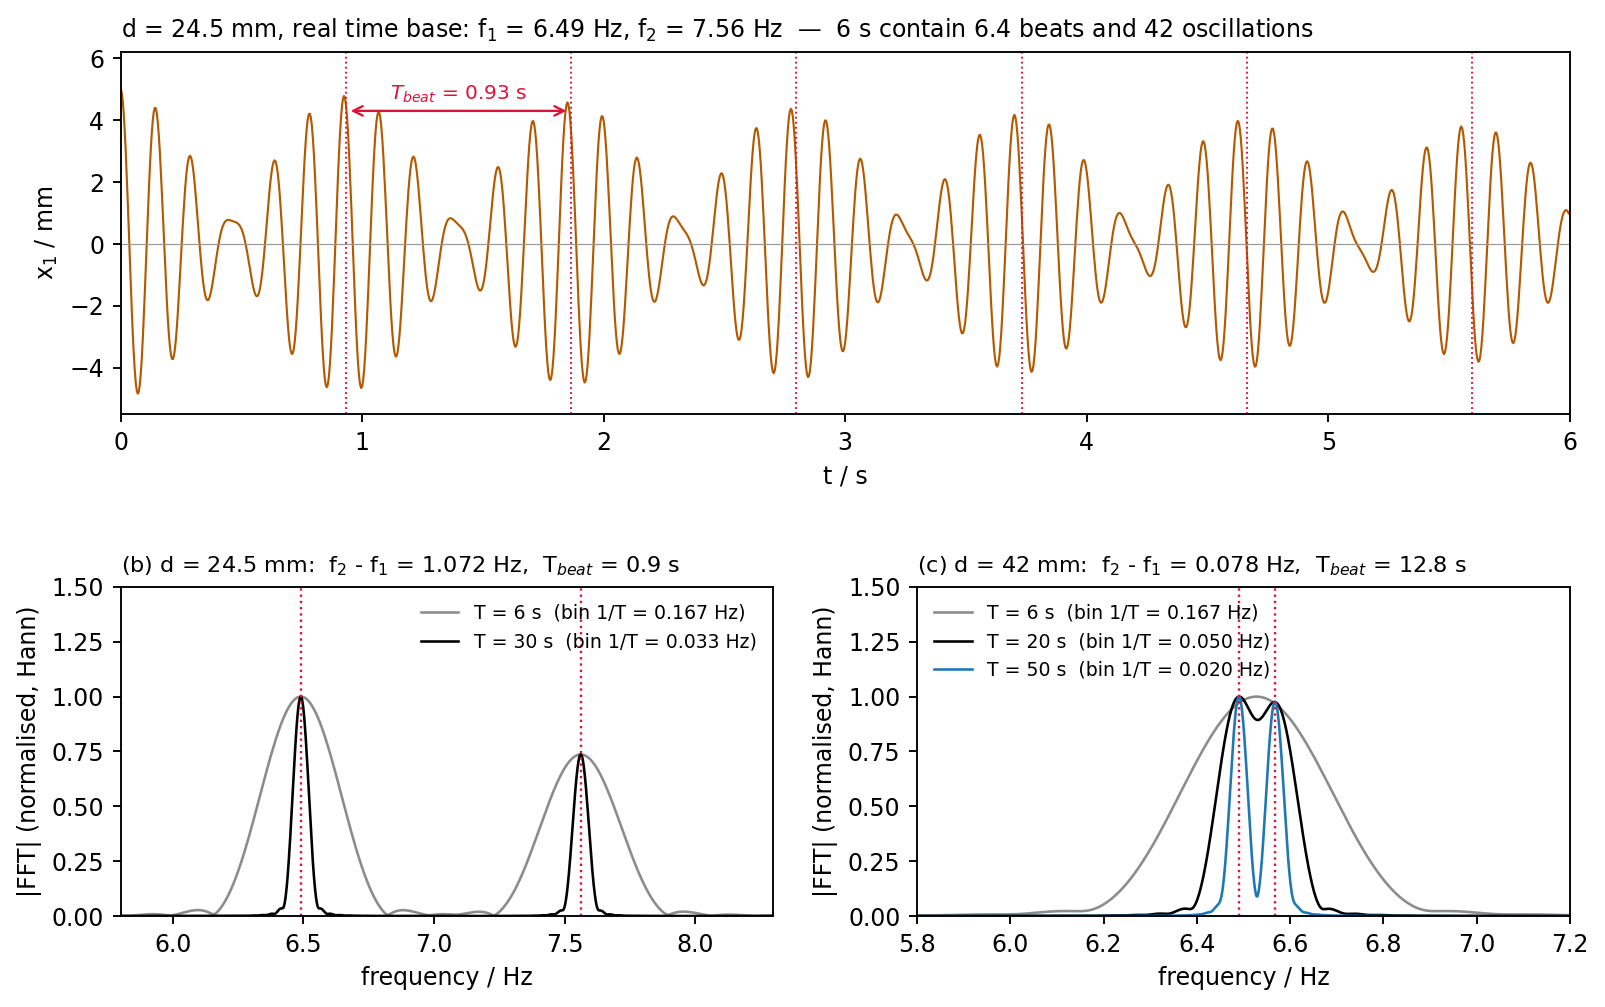
\includegraphics[width=0.7\textwidth]{record_length_real.png}
\caption{Why the record must be longer than 6 s even though 6 s already show six beats. Top: $x_1(t)$ at $d=24.5\un{mm}$ (simulated with the run-1 constants). (b) Spectrum of a 6 s and of a 30 s record at 24.5 mm: both show two peaks, but the 6 s peaks are $0.17\un{Hz}$ wide and their positions are uncertain by a good fraction of that. (c) At 42 mm a 6 s record gives one blob, 20 s a shoulder, 50 s two peaks.}
\end{figure}

\section{The measurement session --- step by step (8 separations $\times$ 5 trials)}

\subsection*{Once per session}
\begin{enumerate}[leftmargin=1.6em,itemsep=1pt]
\item Photograph the set-up with the ruler; note date, room temperature, camera model, fps, distance camera--springs, which strip is ``spring 1'' (mark them with tape; they are never swapped).
\item Measure $L$ (jaw to magnet centre), $b$, $h$ (micrometer, 5 places along the strip), magnet $D$ and $t$, mass $M$ of each magnet with its glue/dot (weigh before gluing, or weigh identical spares), mass of a measured length of strip ($\mu$).
\item \textbf{Tune the pair.} With the magnets far apart ($>70\un{mm}$), film each spring alone for 10 s and read $f_a$, $f_b$ from the Tracker FFT (a stopwatch cannot resolve $1\,\%$ at 6.5 Hz). If they differ by more than $1\,\%$, slide the faster (stiffer) strip a millimetre \emph{up} in its clamp (or the slower one down; $f\propto L^{-3/2}$, so $1\un{mm}$ on $150\un{mm}$ is $1\,\%$) and repeat; then tighten fully and re-measure $L$.
\item \textbf{``Infinity'' videos}: remove magnet 2 (or move spring 2 $>70\un{mm}$ away, where the coupling shifts $f$ by $<0.1\,\%$), pull spring 1 by $5\un{mm}$, record $45\un{s}$; three trials. Same for spring 2 alone. Repeat at the \emph{end} of the session to detect drift.
\end{enumerate}

\subsection*{Per separation (repeat for the 8 values, random order)}
\begin{enumerate}[leftmargin=1.6em,itemsep=1pt]
\item Move clamp 2 to the target spacing (clamp 1 stays); tighten; wait until both springs are at rest.
\item Measure the gap $g$ between magnet faces at rest with a calliper (three readings, do not touch the magnets) or from a photo against the ruler; $d=g+t$.
\item Set the amplitude stop: calliper locked at $5.00\un{mm}$ against the outer face of strip 1, slide the post up to it, fix, remove the calliper (\S3).
\item Camera on, $3\un{s}$ rest, pull strip 1 outwards against the stop, hold $2\un{s}$, release cleanly (open the fingers, do not push), record for the time in the table, stop. Do \emph{not} touch the base while recording.
\item Repeat five times. Between trials wait until both springs are still (about $60\un{s}$ of free decay, or damp them with a finger and wait 10 s; residual motion of spring 2 changes the initial condition).
\item Name files \texttt{d24\_t1.mp4} \dots; keep a log line: file, $g$, $d$, $T$, anything unusual (hand touched, strip tapped the stop, wobble, draught).
\end{enumerate}

\subsection*{More things to watch}
\begin{itemize}[leftmargin=1.6em,itemsep=1pt]
\item \textbf{Both springs at rest before every trial} --- a residual $0.5\un{mm}$ motion of spring 2 changes the mode amplitudes (not the frequencies, but it spoils the peak-ratio test). Damp them by touching both magnets briefly with a finger, then wait 10 s.
\item \textbf{Pull slowly ($\approx1\un{s}$), hold $\approx2\un{s}$}, the same every trial. A slow pull lets spring 2 follow quasi-statically to $x_{20}$; a jerk would leave it ringing with up to $0.8\un{mm}$ amplitude at 24.5 mm, and 2 s of hold damp that by only $10\,\%$ ($\tau\approx21\un{s}$). Pulled over 1 s, the residual ringing is $\approx0.02\un{mm}$.
\item \textbf{Storage}: 40 clips of one minute at 240 fps is $\approx10$--$40\un{GB}$ depending on the phone; check the free space and that no clip is cut short.
\item \textbf{Light flicker}: at 240 fps mains-powered lamps produce a 100 Hz brightness ripple that confuses autotracking. Use daylight or a battery lamp, and a matt background.
\item \textbf{Temperature}: do all 40 videos in one session (about two hours) (Young's modulus and remanence both drift $\sim0.1\,\%$/K); note the room temperature at the start and end.
\item \textbf{Clamp creep}: after the session re-record the ``Infinity'' videos. If $f_1$ moved by more than $0.5\,\%$, treat the drift as a systematic error (interpolate linearly in time between the two calibrations).
\item \textbf{Keep the dots}: the tracked dot must not be repainted or moved between trials; if a magnet is knocked, re-measure $g$.
\item \textbf{Tripod and camera}: don't touch the tripod during recording; use the volume button/remote or a 3 s timer to start; lock focus and exposure.
\end{itemize}

\subsection*{Release with a burnt thread instead of fingers?}
Not needed here. The thread-and-flame release is for \emph{vertical} pendulums where a hand disturbs the plane; for a leaf spring pulled sideways by $5\un{mm}$, letting go with two fingertips gives a clean start, and the analysis window begins $1\un{s}$ later anyway. A thread would also have to be tied at the magnet, exactly where you track. If you prefer a mechanical release, a small wooden wedge pulled away horizontally works.

\section{Instead of a second run: the data-processing comparison}

Repeating the whole grid is not needed if the first run already follows the rules above; the ``method development'' can be done entirely in the analysis, on the same tracks, and it is worth more marks than a second identical run because it isolates the effect of each analysis choice. For every video compute $f_1$, $f_2$ with:
\begin{enumerate}[leftmargin=1.6em,itemsep=1pt]
\item \textbf{Rectangular window, full record} --- the naive FFT; peak positions from the highest bin. Expected uncertainty $\pm\tfrac12\cdot1/T$.
\item \textbf{Rectangular window, first 6 s only} --- reproduces the situation of the first analyses (peaks $0.17\un{Hz}$ wide, merged beyond $\approx33\un{mm}$); shows why $T$ matters.
\item \textbf{Hann window + zero padding} ($N_{\rm FFT}\ge2^{16}$ for $10\,800$ samples) --- suppresses leakage between the two peaks; peak from the interpolated maximum; uncertainty $\approx0.1/T\approx2\un{mHz}$ for a clean peak.
\item \textbf{Normal coordinates} $x_A+x_B$ (only $f_1$) and $x_A-x_B$ (only $f_2$) --- no resolution problem; requires identical springs, so its disagreement with method 3 is itself a measurement of the detuning.
\item \textbf{Two-tone least-squares fit} $x=[a\cos(2\pi f_1t+\phi_1)+b\cos(2\pi f_2t+\phi_2)]\,e^{-t/\tau}$ --- model-based, sharpest, and gives $a/b$ and $\tau$ directly; with $\tau\approx21\un{s}$ the decay factor is not optional here.
\end{enumerate}
Present one table per method (8 rows of mean $\pm$ SD over 5 trials), the resulting ln--ln gradient for each, and the comparison with the theoretical resolution $1/T$; then adopt method 3 (or 4) for the main result and explain why. This replaces ``run 2'' in the write-up, and the amplitude effect (\S3) becomes the non-linear model test in the evaluation.

\section{Static stiffness $k$ (needed once; do it after the videos)}

With $\omega_a^2=(2\pi\times6.49)^2=1660\un{s^{-2}}$ and a moving mass of $3$--$10\un{g}$, $k=m\omega_a^2\approx5$--$17\un{N\,m^{-1}}$: a $2\un{g}$ load deflects the tip by $1$--$4\un{mm}$, so ordinary small masses work. Measure the stiffness that enters the theory --- the strip \emph{vertical}, its magnet on, the other magnet removed --- so that the small gravity term (\S2) is included automatically:
\begin{enumerate}[leftmargin=1.6em,itemsep=1pt]
\item \textbf{Horizontal load over a pulley (standard).} Thread tied round the strip at the magnet centre, over a low-friction pulley, masses $1,2,\dots,10\un{g}$ (weighed, $\pm0.01\un{g}$) hung vertically; the thread must be horizontal. Tip deflection $x$ from a photo against the ruler (or Tracker on the photo, $\pm0.1\un{mm}$), loading and unloading to expose friction and hysteresis. $k$ = gradient of $F=m_{\rm w}g$ against $x$; keep $x\le10\un{mm}$ (linear region, and the amplitude range used in the videos).
\item \textbf{Tilt method (no pulley, friction-free).} Raise one edge of the base on shims of known thickness so that gravity has a component along $x$; $\theta=\arctan(\text{rise}/\text{base width})$. With $k\approx10\un{N\,m^{-1}}$ the tip moves only $\approx0.1\un{mm}$ per degree, so this needs $\theta$ up to $10$--$15^\circ$ and is less convenient here than the pulley --- use it only if no pulley is available. Generalised force for the tip-load shape: $F=g\sin\theta\,(M+0.375\,\mu L)$.
\item \textbf{Dynamic check.} Add known masses $\Delta m=1,2,3\un{g}$ (weighed Blu-Tack) at the magnet and measure $f_a$ each time. Plotting $1/(2\pi f_a)^2$ against $\Delta m$ gives $1/k$ as the gradient and $m/k$ as the intercept --- a second, independent measurement of both $k$ and $m_{\rm eff}$ (the gravity term changes by $1.2g\Delta m/L\approx0.1$--$0.2\un{N\,m^{-1}}$, i.e.\ $1$--$2\,\%$: mention, do not fuss).
\end{enumerate}
Then compare $m_{\rm eff}=k/(2\pi f_a)^2$ with $M+\frac{33}{140}\mu L$, and $k$ with $Ebh^3/4L^3$ (expect the measured value a few per cent lower: gravity, and a clamp is never perfectly rigid).

\textit{Moment of inertia} is not needed: the magnet is treated as a point mass moving with the tip; its rotation contributes $\tfrac12 I\dot\theta^2$ with $\theta\approx1.5x/L$, i.e.\ a fraction $\sim(I/M)(1.5/L)^2\sim(D/L)^2/10\lesssim10^{-3}$ of the kinetic energy. Mention it as a negligible correction, do not measure it.

\section{Data processing checklist}

\begin{enumerate}[leftmargin=1.6em,itemsep=1pt]
\item Tracker: Clip Settings with frame rate \textbf{240} typed in (check dt $=4.17\times10^{-3}\un{s}$ in every clip), start frame $\approx1\un{s}$ after release, end frame $45\un{s}$ later, step size 2; calibration stick; axes with origin on the dot of magnet 1 in a rest frame, $x$ horizontal; point mass A on magnet 1, point mass B on magnet 2 (autotracker); export \texttt{t, x\_A, x\_B} as text.
\item Python: subtract the mean of each track, then the five methods of \S5; beat period from the envelope; peak-height ratios $r_1$, $r_2$ (identical-spring test); actual $A$ from the first maximum; $\tau$ from the envelope.
\item \textbf{Equilibrium of mass B.} $x_B$ oscillates about $\approx d$, not about 0, because the origin sits on magnet 1 --- leave it. Do not move the axes to fix it (that would give the two masses different origins) and do not shift $x_B$ in Tracker. In Python subtract from each track its own mean over the analysed window (over $\ge3$ whole beats the mean of a decaying two-tone signal is its rest position to $\ll0.1\un{mm}$), or subtract the value averaged over the 3 rest seconds before the pull; both give $x_1$, $x_2$ measured from equilibrium as in the theory. Tracker's own FFT ignores the offset anyway (it appears only in the zero-frequency bin, which is why your spectrum is clean).
\item Per $d$: mean and standard deviation of the 5 trials (random error), compared with the FFT uncertainty (systematic floor); take the larger.
\item Graphs: $f_1,f_2$ vs $d$; $\ln(f_2^2-f_1^2)$ vs $\ln d$ with weighted fit (gradient vs $-5$); $f_{\rm avg}$ and $f_{\rm beat}$ vs $d$; residuals; then the non-linear and finite-size models in the evaluation.
\end{enumerate}

\needspace{12\baselineskip}
\section*{Summary card (print and keep at the bench)}
\begin{center}\small
\begin{tabular}{@{}lp{13.5cm}@{}}
\toprule
fps & 240 recorded \textbf{and} typed into Tracker's Clip Settings (dt $=4.17\un{ms}$); step size 2\\
spring & the present strip ($f_a\approx6.5\un{Hz}$) or one $\le15\,\%$ longer; tune $f_a=f_b$ to $<1\,\%$ (Tracker FFT of each spring alone) by sliding one strip in its clamp\\
release & spring 1 pulled \textbf{outwards} against the stop (set once per $d$ with the calliper locked at 5.00 mm), hold 2 s, open the fingertips\\
$d$ & set clamps, then \emph{measure} $g$ with calliper, $d=g+t$; 3 readings\\
record & 3 s rest, slow pull (1 s), hold 2 s, release, then \textbf{45 s} for $d\approx24.5$, 26.5, 28.5, 31, 33.5, 36, 39, 42 mm\\
 & (rule: $T\ge3T_{\rm beat}$ --- 3.5 beats at 42 mm, 48 at 24.5 mm; the 35 s already recorded at 24.5 mm is fine; quote $T$ per point)\\
trials & 5 per $d$, random order of $d$; wait until still between trials\\
also & ``Infinity'' (each spring alone, $>70$ mm apart) $3\times45$ s at start and end; photo of set-up; $L,b,h,M,\mu,D,t$; $k$ by load--deflection (strip vertical, magnet on)\\
never & steel/phone near the magnets; touching the base or tripod during a recording; changing $L$, the dots or the magnet positions during the session\\
\bottomrule
\end{tabular}
\end{center}
\end{document}
